\documentclass{beamer}
\usepackage{graphicx}

\mode<presentation>
{
  \usetheme{Frankfurt}
  \setbeamercovered{transparent}
}

\setcounter{tocdepth}{1}

\title[Water Compression]{Improved Data Compression of Molecular Dynamics of
  Water}

\subtitle{Project Proposal}

\author{Keegan Smith
  \and Julian Kenwood
  \and Min-Young Wu}

\titlegraphic{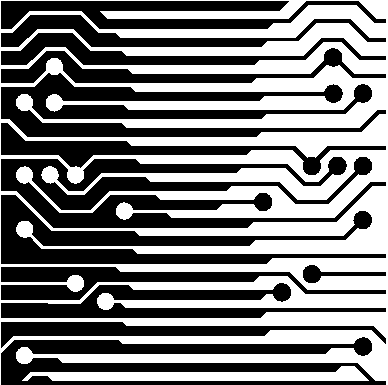
\includegraphics[height=16mm]{cslogo}}

\date{May 22, 2009}

\institute[UCT]{Department of Computer Science \\ University of Cape Town}

\AtBeginSection[]
{
  \begin{frame}
    \frametitle{Outline}
    \tableofcontents[currentsection]
  \end{frame}
}

\begin{document}

\begin{frame}
  \titlepage
\end{frame}


\begin{frame}{Overview}
  \tableofcontents
\end{frame}

\section{Introduction}


\subsection{Intro}
\begin{frame}{Water compression}
  We are implementing a lossless compression algorithm for data generated by
  MD simulations. We are specifically targeting data with large amounts of
  water in the simulation.

  \begin{figure}
    \centering
    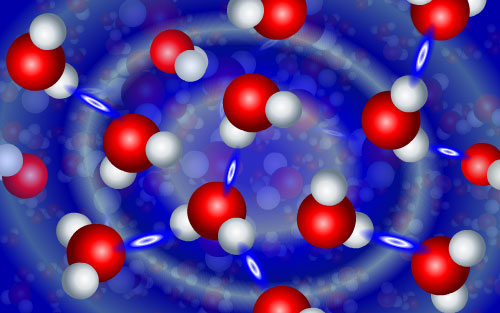
\includegraphics[width=75mm]{water_bonds.jpg}
  \end{figure}
\end{frame}


\subsection{Molecular simulations}
\begin{frame}{Molecular simulations}
 \begin{itemize}
  \item Runs for days (35\,000 frames a day)
  \item Lots of data (1 frame $\approx$ 5 gigabytes of data)
  \item A significant portion of which is water
 \end{itemize}
  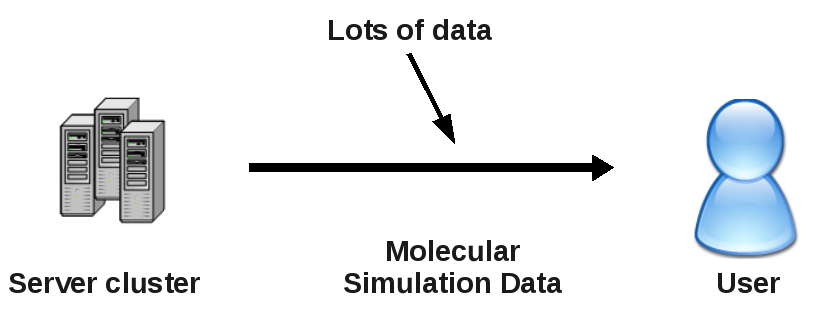
\includegraphics[width=100mm]{data.png}
\end{frame}


\subsection{Compression}
\begin{frame}{Compression}
 \begin{itemize}
  \item General Encoding
  \begin{itemize}
   \item Independent of the underlying structure of data
   \item Huffman Encoding
   \item Arithmetic Coding
   \item gzip/bzip/zip
  \end{itemize}
 \item Domain-Specific Encoding
  \begin{itemize}
   \item Exploits known characteristics of data
   \item MP3/WMA 
   \item MPEG/WMV
   \item XML Compression
  \end{itemize}
 \end{itemize}
\end{frame}


\subsection{Related Work}
\begin{frame}{Related Work}
  \framesubtitle{A look at point cloud compression}
  Point Cloud Compression
  \begin{itemize}
  \item \textbf{Point Cloud} - List of coordinates
  \item Domain-Specific Encoding. Uses layout of points locally and/or
    globally
  \end{itemize}
  MD Point Cloud Compression
  \begin{itemize}
  \item Omeltchenko et al. (2000) use a space filling curve and encode
    differences of positions along curve
  \end{itemize}
\end{frame}


\begin{frame}{Related Work}
  \framesubtitle{A look at point cloud compression}
  Surface Point Cloud Compressors
  \begin{itemize}
  \item Devillers and Gandoin (2000) exploit a property of kd-trees
  \item Gumhold et al. (2005) and Merry et al. (2006) exploit regularity of
    surface scans with \emph{predictors}
  \end{itemize}
  \begin{figure}
    \centering
    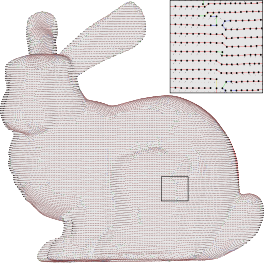
\includegraphics[width=50mm]{bunny}
  \end{figure}
\end{frame}



\section{Approach}


\subsection{Quantisation}
\begin{frame}{Quantisation}
  \begin{itemize}
  \item Receive positions of atoms
  \item Quantise positions
  \item Lossy % TODO 9 Remember to mention this is the only lossy bit of the
              % algorithm. Also mention that quantisation is acceptable loss,
              % so in literature the algorithm in total is still referred to
              % as lossless
  \end{itemize}
  \begin{figure}
    \centering
    \begin{tabular}{cp{4mm}c}
      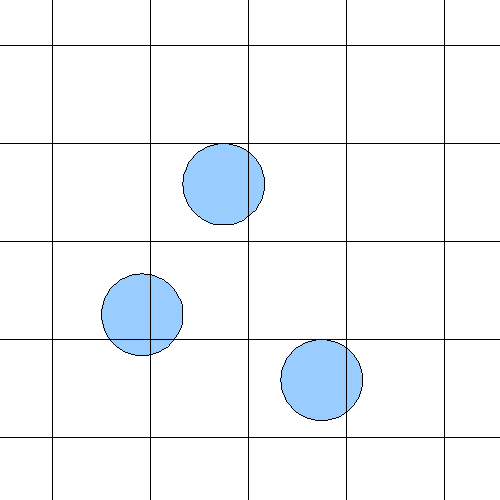
\includegraphics[width=30mm]{unquantised} & &
      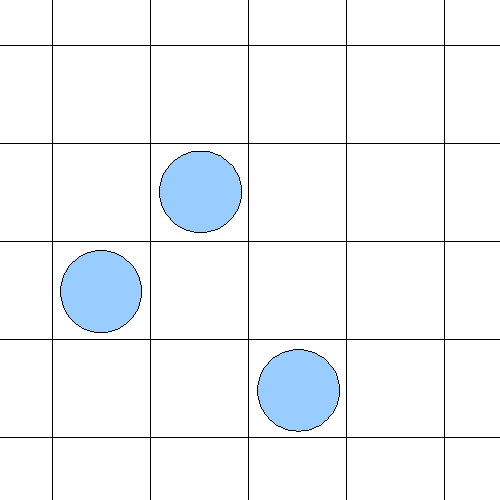
\includegraphics[width=30mm]{quantised} \\
      Floating Point & & Quantised
    \end{tabular}
  \end{figure}
\end{frame}


\subsection{Single-Frame Compression}
\begin{frame}{Single-Frame Compression}
  \begin{itemize}
  \item Find water molecules (bond extraction)
  \item Connect water molecules (graph)
  \item Create rooted spanning tree
  \item Use predictors to predict next water molecule
  \item Encode predictor and error (compression)
  \end{itemize}
  \begin{figure}
    \centering
    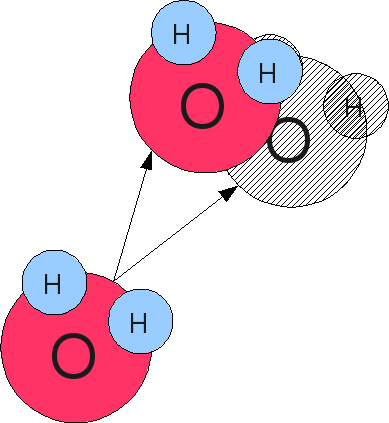
\includegraphics[height=30mm]{prediction}
  \end{figure}
\end{frame}


\subsection{Other}
\begin{frame}{Other}
  \begin{itemize}
  \item Inter-frame Prediction
    \begin{itemize}
    \item Prediction using last $n$ frames
    \item Most atoms don't move much
    \item Single frame compression computationally expensive
    \item Inter-frame encoding much faster
    \end{itemize}
  \item Visualisation
    \begin{itemize}
    \item Quantisation level is an input parameter
    \item Clutter Reduction Techniques
    \end{itemize}
  \end{itemize}
\end{frame}



\section{Plan}


\subsection{Project Plan}
\begin{frame}{Project Plan}
  \begin{itemize}
  \item Visualisation
    \begin{itemize}
    \item Quantisation
    \item Visualisation
    \end{itemize}
  \item Connectivity
    \begin{itemize}
    \item Bond extraction
    \item Constructing graph connecting water molecules
    \end{itemize}
  \item Compression
    \begin{itemize}
    \item Encoding initial spanning tree
    \item Inter-frame compression
    \end{itemize}
  \end{itemize}
\end{frame}


\subsection{Research Questions}
\begin{frame}{Research Questions}
  \uncover<1>{
  Visualisation
  \begin{itemize}
    \item Acceptable level of quantisation?
    \item Effectively visualise and cope with large levels of detail?
  \end{itemize}}

  \uncover<2>{
  Connectivity
  \begin{itemize}
    \item Exploit what we know about water?
    \item Can we improve on other methods?
    \begin{itemize}
      \item Devillers and Gandoin
      % progressive point cloud compression using octrees
      \item Na\"ive graph using heuristics
    \end{itemize}
  \end{itemize}}

  \uncover<3>{
  Compression
  \begin{itemize}
    \item Space and time efficiencies?
    \item Achieve better compression rates than other methods?
    \begin{itemize}
      \item Omeltchenko et al.
      % space filling curve
      % - assign coords, sort, encode
    \end{itemize}
  \end{itemize}}
\end{frame}



\subsection{Breakdown}
\begin{frame}{Work Breakdown}
  \framesubtitle{Single Frame Compressor}
  \begin{figure}
    \centering
    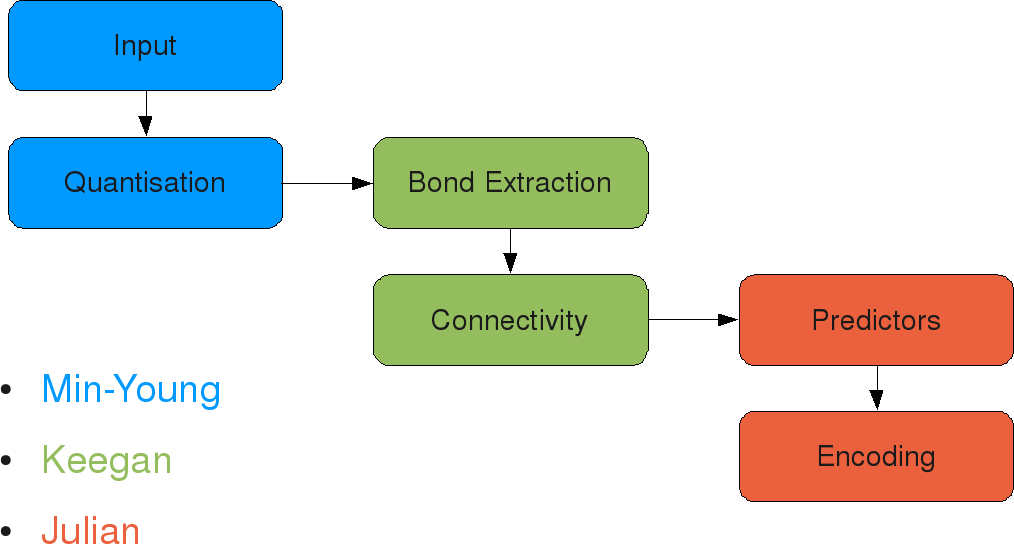
\includegraphics[width=100mm]{breakdown}
  \end{figure}
\end{frame}


\subsection{Interfaces}
\begin{frame}{Interfaces Between Components}
  \framesubtitle{Single Frame Compressor}
  \begin{figure}
    \centering
    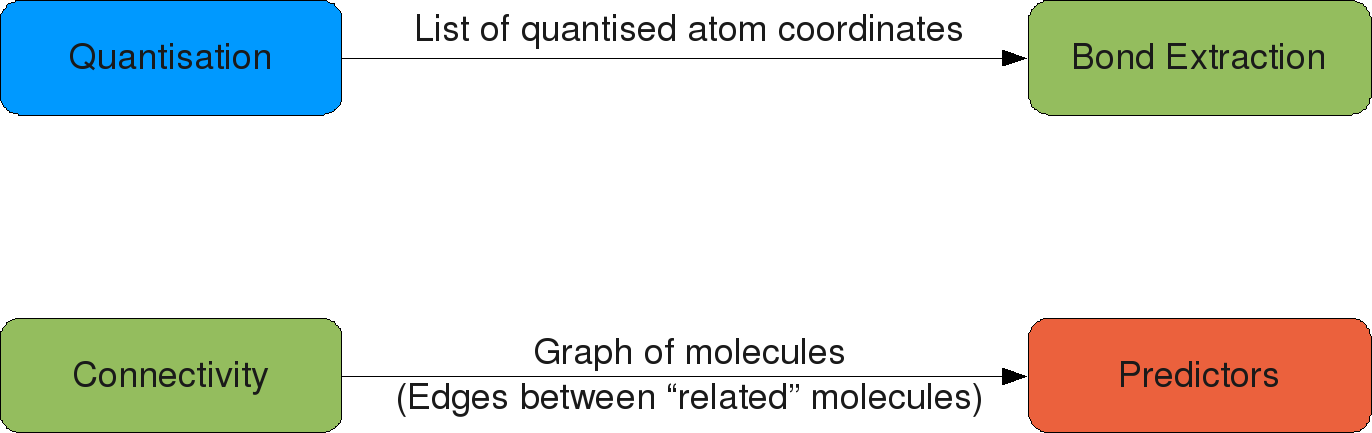
\includegraphics[width=100mm]{interfaces}
  \end{figure}
\end{frame}


\subsection{Other Work Breakdown}
\begin{frame}{Work Breakdown}
  \framesubtitle{Other}
  \begin{itemize}
  \item Min-Young
    \begin{itemize}
    \item Visualisation
    \item Quantisation Experimentation
    \end{itemize}
  \item Keegan
    \begin{itemize}
    \item Theoretical Analysis of the Compression Algorithm
    \end{itemize}
  \item Julian
    \begin{itemize}
    \item Inter-frame Compression
    \item Reference Implementations
    \end{itemize}
  \end{itemize}
\end{frame}


\subsection{Risks}
\begin{frame}
  \frametitle{Risks}
  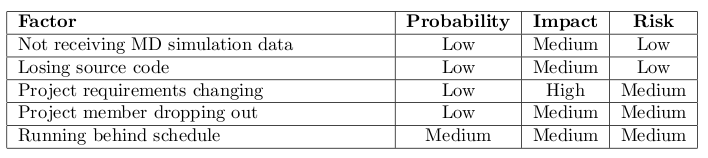
\includegraphics[width=100mm]{risks}    
\end{frame}


\subsection{Resources}
\begin{frame}
  \frametitle{Resources Required}
  \begin{itemize}
  \item MD Simulation Data
  \item Implemented in C++ on GNU/Linux
    \begin{itemize}
    \item Arithmetic Encoding Library
    \item OpenGL
    \end{itemize}
  \item Developed on Home and Lab Machines
  \item People
  \end{itemize}
\end{frame}



\section{Anticipated Outcomes}


\subsection{Deliverables and Milestones}
\begin{frame}
  \frametitle{Deliverables and Milestones}
  \begin{itemize}
  \item Software to visualise MD data
  \item Compression Program
    \begin{itemize}
    \item \emph{Milestone 1} - na\"ive compression
    \item \emph{Milestone 2} - single-frame compression
    \item \emph{Milestone 3} - inter-frame compression
    \end{itemize}
  \item Decompression Program
    \begin{itemize}
    \item Part of Milestone 2 and 3
    \end{itemize}
  \end{itemize}
\end{frame}


\subsection{Key Success Factors}
\begin{frame}{Key Success Factors}
  \uncover<1>{
    Visualisation Key Success Factors
    \begin{itemize}
    \item Quantitative evaluation of quantisation levels
      % explain: can the difference be seen
    \item Acceptable quantisation levels determined via user testing
    \item Effective visualisation of molecular simulations
      % \item Acceptable quantisation levels implemented in the system
    %\item TODO 10 Metrics for user testing
    \end{itemize}
  }

  \uncover<2>{
    Connectivity Key Success Factors
    \begin{itemize}
    \item Achieve better compression ratios in the context of point cloud
      compression
    \item Do we compress efficiently
    \item Do we decompress efficiently
    \end{itemize}
  }

  \uncover<3>{
    Compression Key Success Factors
    \begin{itemize}
    \item Achieve better compression ratios in the context of space and time
      requirements
    \item Do we achieve better compression rates than other schemes
   \end{itemize}
  }
\end{frame}


\subsection{Issues}
\begin{frame}{Ethical, Professional and Legal Issues}
  \begin{itemize}
   \item User experiments
   \item Open Source
    \begin{itemize}
     \item Likely to be included in VMD software package
    \end{itemize}
  \end{itemize}
\end{frame}


\subsection{Conclusion}
\begin{frame}{Conclusion}
  \begin{itemize}
  \item We hope we shown that our project\dots
    \begin{itemize}
    \item \dots presents a solution to a problem that needs to be solved
    \item \dots is well thought out in terms of the approach
    \item \dots has a fair work breakdown for each member
    \item \dots has minimal unmitigated risks
    \end{itemize}
  \end{itemize}
\end{frame}


\begin{frame}{Questions}
 \begin{center}
  \item Any Questions?
 \end{center}
\end{frame}


\end{document}
